\documentclass[a4paper, 12pt]{article}
\usepackage[a4paper,top=1.5cm, bottom=1.5cm, left=1cm, right=1cm]{geometry}

% Работа с русским языком
\usepackage[utf8]{inputenc}
\usepackage{mathtext}                % русские буквы в формулах
\usepackage[english, russian]{babel} % локализация и переносы

\usepackage{graphicx}   % Вставка изображений
\usepackage{float}      % "Плавающие" изображения3
\usepackage{wrapfig}    % Обтекание фигур (таблиц, картинок и прочего)
\usepackage{subfig}
\graphicspath{ {./images/} }

\usepackage{tabularx}
\usepackage{multirow}
\usepackage{amsmath}
\usepackage{amsfonts}
\usepackage{indentfirst}
\usepackage{longtable}
\graphicspath{{pictures/}}
\usepackage{natbib}
\usepackage{bm}

%%% Колонтитулы
\usepackage{titleps}
\newpagestyle{main}{
	\setheadrule{0.4pt}
	\sethead{Магнитометр}{}{}
	\setfootrule{0.4pt}                       
	\setfoot{ФРКТ МФТИ, 2023}{}{\thepage} 
}
\pagestyle{main}  

\begin{document}
    \begin{titlepage}
	\begin{center}
            {\large МОСКОВСКИЙ ФИЗИКО-ТЕХНИЧЕСКИЙ ИНСТИТУТ (НАЦИОНАЛЬНЫЙ ИССЛЕДОВАТЕЛЬСКИЙ УНИВЕРСИТЕТ)}
	\end{center}
 
	\begin{center}
		{\large Физтех-школа радиотехники и компьютерных технологий}
	\end{center}
	
	\vspace{8cm}
	{\LARGE
		\begin{center}
                {\bf Отчёт о выполнении лабораторной работы 3.1.1}\\
                Магнитометр
		\end{center}
	}
	\vspace{5cm}
	\begin{flushright}
		{\Large Автор:\\ Тихонов Дмитрий Романович, \\
			\vspace{0.2cm}
			студент группы Б01-206}
	\end{flushright}
	\vspace{5cm}
	\begin{center}
		\Large Долгопрудный, 2023
	\end{center}
    \end{titlepage}


    \section{Введение}

    \noindent \textbf{Цель работы:} определить горизонтальную составляющую магнитного поля Земли и установить количественное соотношение между единицами электрического тока в системах СИ и СГС. \\

    \noindent \textbf{В работе используются:} магнитометр, осветитель со шкалой, источник питания, вольтметр, электромагнитный переключатель, конденсатор, намагниченный стержень, прибор для определения периода крутильных колебаний, секундомер, рулетка, штангенциркуль.
    
    \section{Теоретические сведения и методика измерений}

    \subsection{Экспериментальная установка}

    \textit{Магнитометром} называют прибор для магнитных измерений. В нашей установке используется электромагнитный магнитометр (рис. \ref{magnetometer}), который состоит из нескольких последовательно соединённых круговых витков К, расположенных вертикально. В центре кольца К радиусом $R$ на тонкой неупругой вертикальной нити подвешена короткая магнитная стрелка С. Жёстко связанная со стрелкой крыльчатка погружена в масло и служит для демпфирования колебаний.

    \begin{figure}[H]
        \centering
        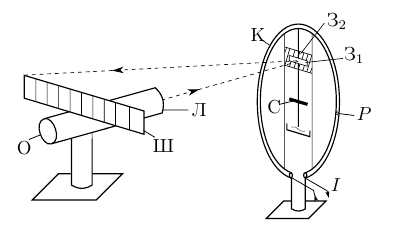
\includegraphics{images/magnetometer.png}
        \caption{Схема магнитометра}
        \label{magnetometer}
    \end{figure}

    В отсутствие других магнитных полей стрелка располагается по направлению горизонтальной составляющей земного магнитного поля $\bm{B}_0$, т. е. лежит в плоскости магнитного меридиана.

    Прибор настраивают с помощью световых зайчиков, отражённых от двух зеркал: $\text{З}_1$, прикреплённого к стрелке (подвижный зайчик), и $\text{З}_2$, расположенного в плоскости кольца К и жёстко связанного с ним (неподвижный зайчик). Оба зеркала освещаются одним и тем же осветителем О. Вращением кольца вокруг вертикальной оси можно совместить оба зайчика. При этом плоскость витков совпадает с плоскостью магнитного меридиана.
    
    При появлении дополнительного горизонтального магнитного поля $\bm{B}_\perp$ стрелка С установится по равнодействующей обоих полей $\bm{B}_\Sigma$ (рис. \ref{installation}). В нашей установке дополнительное поле может быть создано либо малым ферромагнитным стержнем, расположенным на кольце на его горизонтальном диаметре ($\bm{B}_1$), либо током, проходящим по кольцу ($\bm{B}_2$). В обоих случаях дополнительное поле можно считать однородным, так как размеры стрелки много меньше радиуса кольца.
    
    Поле намагниченного стержня вдали от него может быть приближённо вычислено как поле точечного диполя:

    \begin{equation}
        \bm{B}(\bm{r}) = \frac{\mu_0}{4\pi} \left( \frac{3(\bm{\mathfrak{m}} \cdot \bm{r}) \bm{r}}{r^5} - \frac{\bm{\mathfrak{m}}}{r^3} \right),
    \end{equation}

    где $\bm{\mathfrak{m}}$ -- магнитный момент стержня, $\bm{r}$ -- радиус-вектор, проведённый из центра диполя в точку наблюдения. 

    \begin{figure}[H]
        \centering
        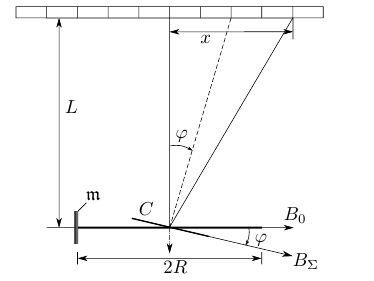
\includegraphics{images/installation.png}
        \caption{Схема измерения угла отклонения магнитной стрелки}
        \label{installation}
    \end{figure}
    
    На оси, перпендикулярной стержню, имеем

    \begin{equation}
        B_1 = \frac{\mu_0}{4\pi} \frac{\mathfrak{m}}{R^3},
        \label{eq:dipole_field}
    \end{equation}

    где $R$ -- радиус кольца.

    Магнитное поле в центре кольца с током $I$ по закону Био-Савара-Лапласа равно

    \begin{equation}
        B_2 = \frac{\mu_0 I}{2R}N,
        \label{eq:ring_current}
    \end{equation}

    где $I$ -- сила тока в единицах СИ, $N$ -- число витков в кольце.

    Измерив угол отклонения $\varphi$, можно связать поля $B_0$ и $B_\perp$:

    \begin{equation}
        B_\perp = B_0 \cdot \tg{\varphi}.
        \label{eq:relationship_B}
    \end{equation}

    \subsection{Определение горизонтальной составляющей магнитного поля Земли}

    Для определения горизонтальной составляющей земного магнитного поля $B_0$ тонкий короткий намагниченный стержень устанавливается в отверстие Р на горизонтальном диаметре кольца (рис. \ref{magnetometer}). Измерив тангенс угла отклонения стрелки

    \begin{equation}
        \tg{\varphi_1} = \frac{x_1}{2L},
        \label{eq:deviation_arrow}
    \end{equation}
    
    можно с помощью уравнений (\ref{eq:dipole_field}), (\ref{eq:relationship_B}) и (\ref{eq:deviation_arrow}) рассчитать поле $B_0$, если исключить величину $\mathfrak{m}$ -- магнитный момент стержня.
    
    Для исключения магнитного момента предлагается измерить период крутильных колебаний стержня в поле Земли. Подвешенный горизонтально за середину на тонкой длинной нити стержень в положении равновесия установится по полю Земли (упругость нити пренебрежимо мала). Если ось стержня отклонить в горизонтальной плоскости от направления $B_0$ на малый угол $\alpha$, то под действием возвращающего механического момента

    \begin{equation}
        M_\text{мех} = \lvert \bm{\mathfrak{m}} \times \bm{B} \rvert = \mathfrak{m} B_0 \sin{\alpha} \approx \mathfrak{m} B_0 \alpha
    \end{equation}
    
    стержень с моментом инерции $J$ в соответствии с уравнением $J \Ddot{\alpha} + \mathfrak{m} B_0 \alpha = 0$ будет совершать крутильные колебания с периодом

    \begin{equation}
        T = 2\pi \sqrt{\frac{J}{\mathfrak{m} B_0}}.
    \end{equation}

    Момент инерции цилиндрического стержня относительно оси вращения

    \begin{equation}
        J = m \left( \frac{l^2}{12} + \frac{r^2}{4} \right) = \frac{ml^2}{12} \left[1 + 3\left( \frac{r}{l}\right)^2 \right],
    \end{equation}
    
    где $m$ -- масса стержня, $l$ -- длина, а $r$ -- его радиус.

    Таким образом, рассчитав момент инерции $J$ и измерив тангенс угла отклонения стрелки $\varphi_1$ и период малых крутильных колебаний стержня $Т$, можно определить горизонтальную составляющую магнитного поля Земли:

    \begin{equation}
        B_0 = \frac{2\pi}{TR}\sqrt{\frac{\mu_0 JL}{2\pi R x_1}} \hspace{4mm} \text{[ед. СИ]}.
    \end{equation}
    
    Поскольку магнитометр установлен в железобетонном здании, магнитное поле в нём может не только сильно отличаться от поля Земли, но и заметно меняться от места к месту, поэтому период колебаний следует измерять непосредственно вблизи магнитометра. Кроме того, для обеспечения максимальной однородности магнитного поля в области измерений следует удалить на максимальное расстояние возможные источники сильного магнитного поля.

    
    \subsection{Определение электродинамической постоянной}
    
    Ток в цепи кольца можно измерить двумя независимыми способами: по магнитному действию тока на стрелку магнитометра и по заряду, протекающему через цепь в единицу времени. Первый способ измерения соответствует тому, как эталон тока определён в системе СИ, а второй в СГС. По отношению результатов этих измерений можно определить электродинамическую постоянную $c$.
    
    Пропуская некоторый ток через витки магнитометра, измерим тангенс угла отклонения стрелки ($\tg{\varphi_2} = x_2/2L$) и по формулам (\ref{eq:ring_current}) и (\ref{eq:relationship_B}) рассчитаем силу тока:

    \begin{equation}
        I = \frac{2B_0 R}{\mu_0 N} \tg{\varphi_2} \hspace{4mm} \text{[ед. СИ]}.
        \label{eq:current_SI}
    \end{equation}

    Тот же ток можно измерить абсолютным образом по прошедшему в единицу времени заряду, что соответствует определению эталона тока в СГС. Если разрядить конденсатор известной ёмкости $C$, заряженный до напряжения $U$, через витки, то через них протечёт заряд $q = CU$ (рис. \ref{circuit}). Если $\nu$ раз в секунду последовательно заряжать конденсатор от источника и разряжать через витки, то через них за секунду протечёт заряд $CU\nu$. Средний ток, прошедший через витки, равен при этом

    \begin{equation}
        I = CU\nu \hspace{4mm} \text{[абс. ед.]}.
        \label{eq:current_ABS}
    \end{equation}

    \begin{figure}[H]
        \centering
        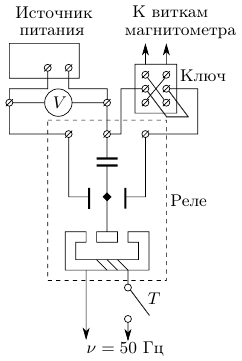
\includegraphics[scale = 0.8]{images/circuit.png}
        \caption{Схема питания катушки магнитометра}
        \label{circuit}
    \end{figure}

    Таким образом, абсолютное измерение тока сводится к нахождению величин $С$ и $U$, которые тоже могут быть определены абсолютным образом.
    
    Итак, для вычисления абсолютного значения тока по (\ref{eq:current_ABS}) необходимо измерить напряжение $U$ на конденсаторе известной ёмкости $С$. Напряжение необходимо выразить в \textit{единицах СГС}. Емкость конденсатора $С$ должна быть выражена в сантиметрах.
    
    По отношению численных значений одного и того же тока, выраженных в единицах СИ и СГС по формулам (\ref{eq:current_SI}) и (\ref{eq:current_ABS}) соответственно, можно определить значение электродинамической постоянной:

    \begin{equation}
        c \left[ \frac{\text{м}}{с} \right] = \frac{1}{10} \frac{I_{\text{[СГС]}}}{I_\text{[СИ]}}.
    \end{equation}

    \section{Результаты измерений и обработка данных}

    \subsection{Измерение горизонтальной состовляющей магнитного поля Земли}

    \begin{enumerate}
        \item Включим осветитель и получим на горизонтальной шкале два чётких световых \textit{зайчика}. Плавным поворотом кольца К (рис. \ref{magnetometer}) вокруг вертикальной оси совместим зайчики.

        \item В отверстие P на горизонтальном диаметре кольца (рис. \ref{magnetometer}) вставим намагниченный стержень и измерим смещение подвижного зайчика $x_1$ (рис. \ref{installation}):

        $$
        x_1 = \left( 0.6 \pm 0.1 \right) \text{ см}.
        $$
        
        Поменяв ориентацию стержня, измерим отклонение зайчика в другую сторону $x_1'$:

        $$
        x_1' = \left(  -3.0 \pm 0.1 \right) \text{ см}.
        $$
        
        Усредняя результаты, получим:

        $$
        \overline{x} = \frac{x_1 - x_1'}{2} = \left( 1.75 \pm 0.05 \right) \text{ см}.
        $$

        \item Измерим расстояние $L$ от шкалы до зеркала:

        $$
        L = \left( 96 \pm 1 \right) \text{ см}.
        $$

        \item Измерим период малых колебаний стержня $T$ в магнитном поле Земли. Для этого поставим стеклянный сосуд \textit{вблизи} магнитометра и опустим на дно привязанный за середину намагниченный стержень.

        $$
        t = \left( 217 \pm 1 \right) \text{ с}, \hspace{1mm} N = 10 \Rightarrow T = \frac{t}{N} = \left( 21.7 \pm 0.1 \right) \text{ с}.
        $$

        \item С помощью штангенциркуля измерим линейные размеры стержня. Кроме того, запишем его массу и параметры магнитометра:

        $$
        m = 4.350 \text{ г}, \hspace{4mm} d = \left( 0.40 \pm 0.01 \right) \text{ см}, \hspace{4mm} l = \left( 4.00 \pm 0.01 \right) \text{ см}, \hspace{4mm} R = 20 \text{ см}.
        $$

        \item Рассчитаем величину горизонтальной составляющей магнитного поля Земли $B_0$ и оценим погрешность результата:

        $$
        J = \frac{ml^2}{12} \left[ 1 + 3 \left( \frac{d}{2l} \right)^2 \right] = \left( 5.8 \pm 0.2 \right) \cdot 10^{-7} \text{ кг} \cdot \text{м}^2,
        $$

        $$
        B_0 = \frac{2\pi}{TR}\sqrt{\frac{\mu_0 JL}{2\pi R\bar{x}}} = \left( 8.2 \pm 0.2 \right) \cdot 10^{-6} \ [ед. СИ].
        $$    
    \end{enumerate}

    \subsection{Определение электродинамической постоянной}

    \begin{enumerate}
        \item Уберём намагниченный стержень из гнезда магнитометра и соберём электрическую схему, изображённую на рис. \ref{circuit}.

        \item Убедимся, что зайчики совмещены в отсутствие тока через витки.

        \item Включим в сеть источник питания и установим рабочее напряжение $U \approx 90$ В.

        \item Замкнув ключ, подключим к цепи витки магнитометра.

        \item Включив кнопкой К электровибратор, измерим напряжение $U$ на конденсаторе и отклонение $x_2$ зайчика на шкале. Поменяв полярность, повторим измерения.

        $$
        x_2 = (-12.5 \pm 0.1) \text{ см}, \hspace{1mm} x_2' = (16.6 \pm 0.1) \text{ см} \Rightarrow \overline{x} = \frac{x_2' - x_2}{2} = \left( 14.55 \pm 0.05 \right) \text{ см}
        $$

        \item Запишем характеристики приборов и параметры $N$, $C$ и $\nu$, указанные на установке:

        $$
        N = 44, \hspace{4mm} C = \left( 9.0 \pm 0.2 \right) \cdot 10^5 \text{ см}, \hspace{4mm} \nu = 50 \text{ Гц}.
        $$

        \item Рассчитаем токи по формулам (\ref{eq:current_SI}) и (\ref{eq:current_ABS}):

        $$
        I_{[СИ]} = \frac{2 B_0 R}{\mu_0 N} \cdot \frac{\bar{x}}{2L} = \left( 4.5 \pm 0.1 \right)\cdot 10^{-3}\ [ед. СИ],
        $$

        $$
        I_{[СГС]} = CU\nu = \left( 1.35 \pm 0.03 \right) \cdot 10^7 \ [ед. СГС].
        $$

        Наконец, вычислим \textit{электродинамическую постоянную} $c$:

         $$
         \boxed{c \ \left[\frac{м}{с}\right] = \frac{1}{10} \frac{I_{[СГС]}}{I_{[СИ]}} = \left( 3.0 \pm 0.1 \right) \cdot 10^8 \text{ м/с}}.
         $$
    \end{enumerate}
    
    \section{Заключение}

    В результате выполнения лабораторной работы получили значение электродинамической постоянной $c = \left( 3.0 \pm 0.1 \right) \cdot 10^8 \text{ м/с}$, что, с учётом погрешности, сходится с табличным значением $c_\text{табл} = 2.998 \cdot 10^8 \text{ м/с}$.

    Неточность в измерении может быть связана с влиянием разных источников магнитного поля (источники питания, токонесущие провода, сотовые телефоны, металлические предметы и т.п.). 

\end{document}